\chapter{Een semantiek voor UML-klassediagrammen en controle op consistentie}\label{sec:consistentie}
In dit hoofdstuk geven we een beschrijving van de verscheidene componenten in een klassediagram die we beschouwen in deze masterproef. Die beschrijving gebruiken we om een modelsemantiek te defini\"eren voor klassediagrammen alsook consistentie en inconsistentie van een klassediagram. We beschrijven ook een methode om een voorstellingswijze voor klassediagrammen in FO($\cdot$) te bekomen die overeenkomt met die semantiek.

\section{Componenten van een klassediagram}\label{sec:cd-components}

We gebruiken figuren \ref{fig:voorbeeld1} en \ref{fig:voorbeeld2} ter illustratie van de componenten in een klassediagram, die we beschrijven in de volgende subsecties.

\begin{figure}[h]
	\centering
	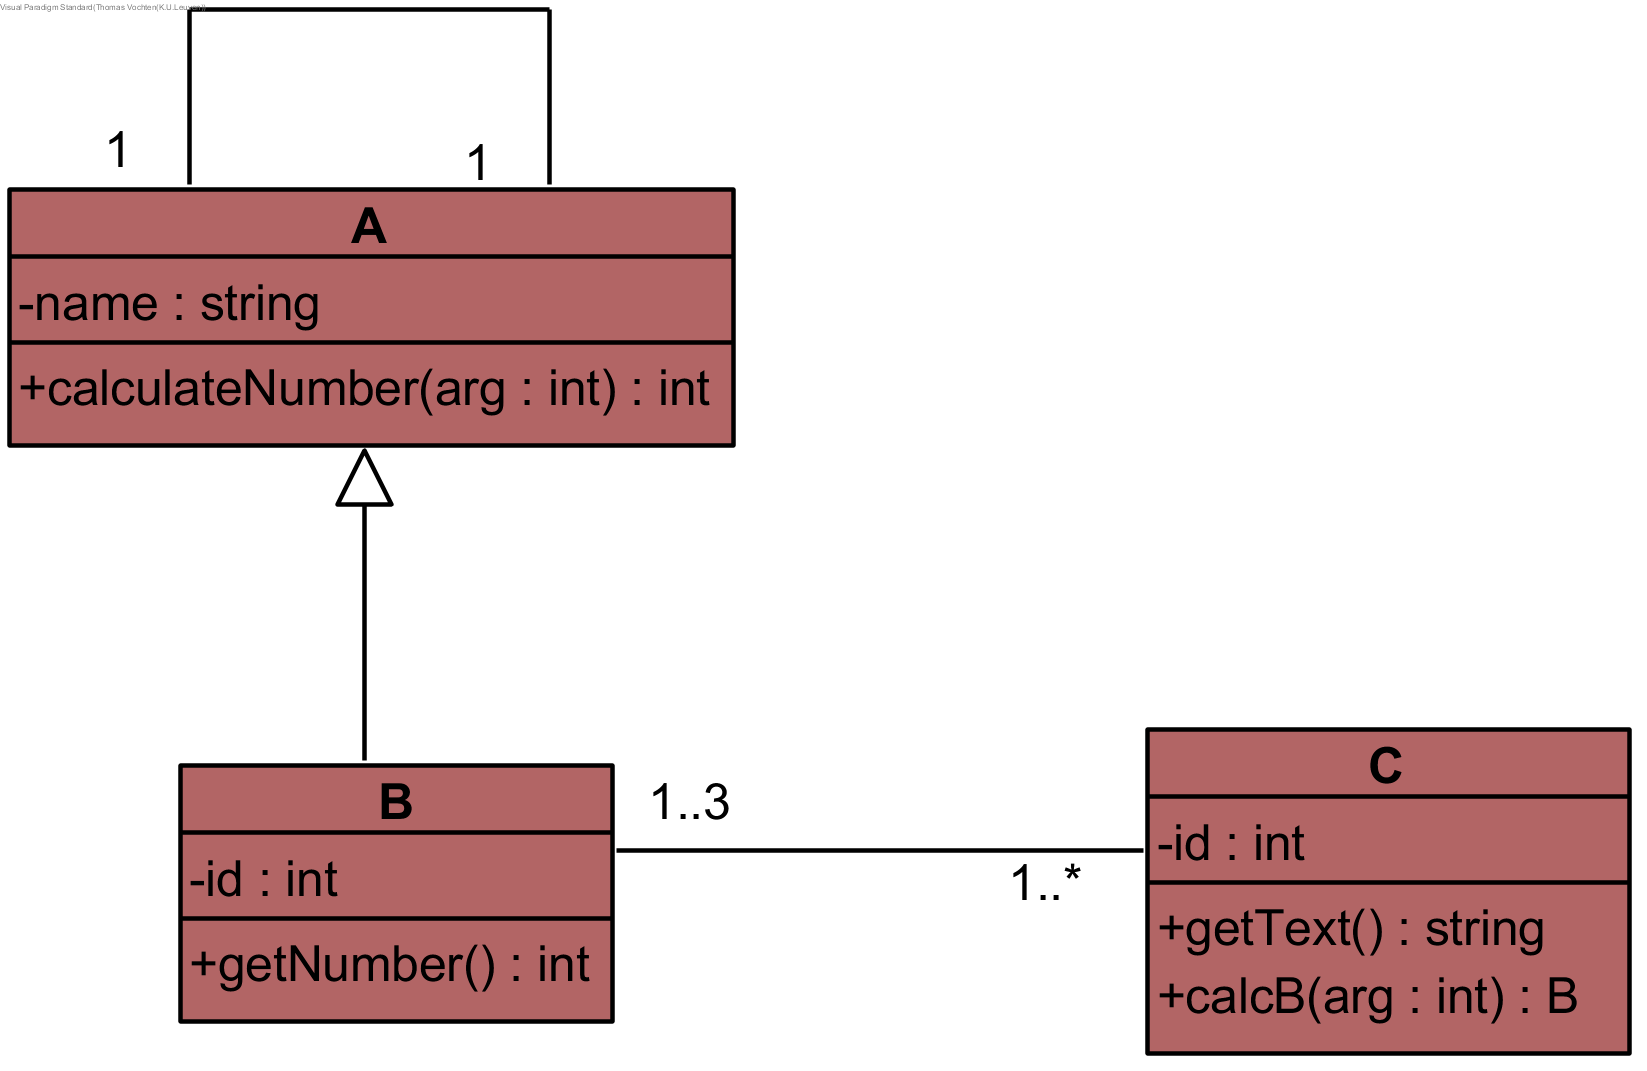
\includegraphics[width=0.6\textwidth]{chap-consistentie/voorbeeld1.png}
	\caption{Klasses, associaties en generalisaties}
	\label{fig:voorbeeld1}
\end{figure}

\begin{figure}[h]
	\centering
	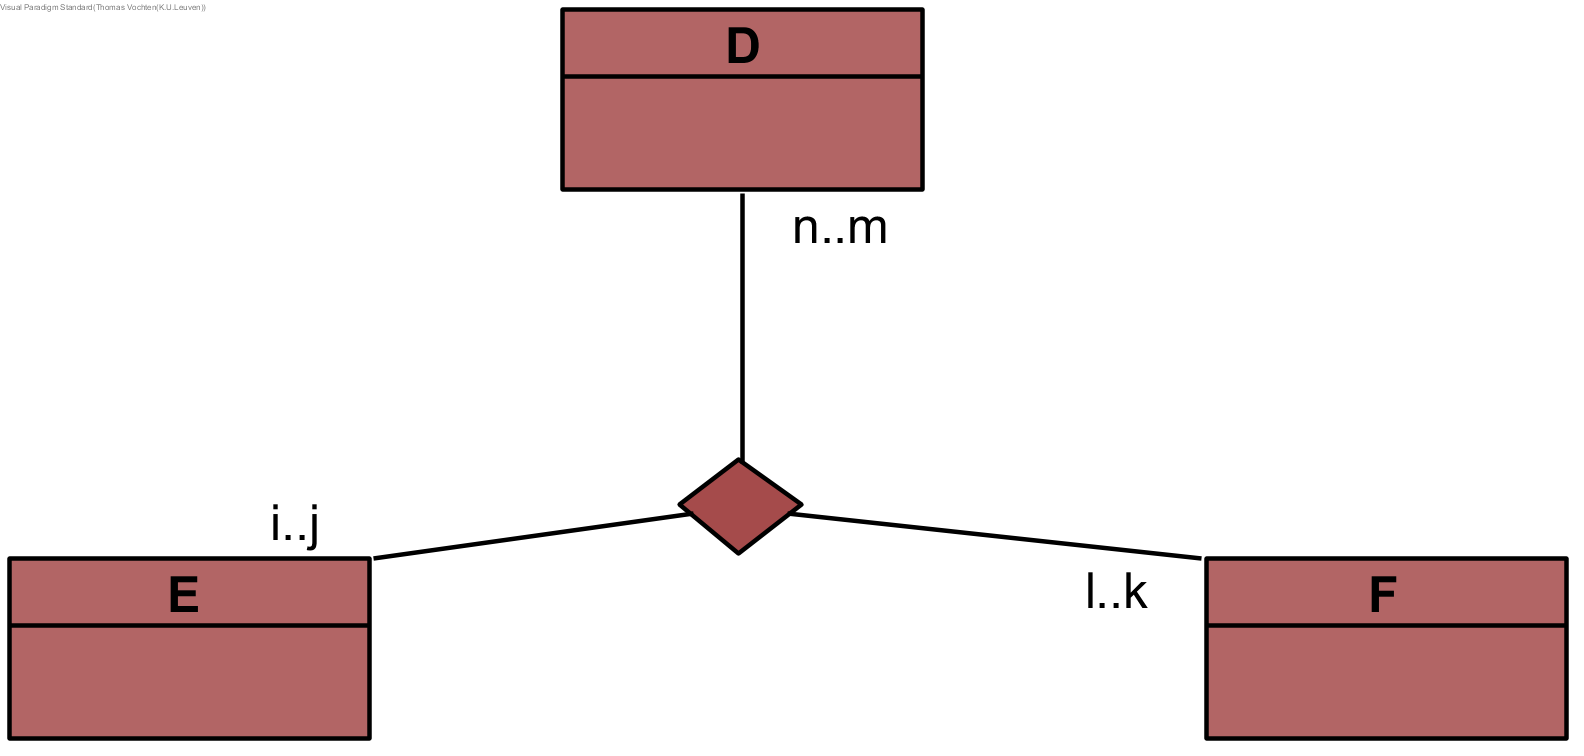
\includegraphics[width=0.6\textwidth]{chap-consistentie/voorbeeld2.png}
	\caption{Meervoudige associaties}
	\label{fig:voorbeeld2}
\end{figure}

\subsection{Klasse}

Klassediagrammen beschrijven de mogelijke structuur van de toestand van een object in het gemodelleerde probleemdomein en welke bewerkingen er beschikbaar zijn op een object. \textbf{Klasses} bepalen hoe die structuur eruit ziet voor een object en benoemt de bewerkingen. We zeggen dat een object een \textbf{instantie} is van een klasse als de toestand van en bewerkingen beschikbaar op dat object overeenkomen met die klasse. Dit concept defini\"eren we preciezer later in deze sectie.

Een klasse bestaat uit de volgende elementen:

\begin{itemize}
	\item Elke klasse heeft een unieke \textbf{naam} binnen eenzelfde klassediagram.
	\item \textbf{Attribuut}: De toestand van een klasse bestaat uit de combinatie van zijn attributen. Elk attribuut heeft een naam en een type. De type van een attribuut kan zowel een primitief type zijn zoals \textit{int} of \textit{string} of een andere klasse uit het diagram, al is dit tweede niet gebruikelijk. Klasse \textit{A} in figuur \ref{fig:voorbeeld1} heeft \textit{name} als attribuut met als type \textit{string}. Een attribuut kan ook een multipliciteit hebben, genoteerd als $n..m$ waarvoor $n,m \in \mathbb{N}$ en $n \leq m$. Dit betekent dat een attribuut minimaal $n$ verschillende waarden heeft en maximaal $m$ verschillende waarden. In de plaats van een bovengrens kan er ook $*$ staan, wat betekent dat een attribuut een arbitrair aantal aan verschillende waarden kan hebben. Indien de ondergrens 0 is, kan het zijn dat er geen waarde bestaat voor die attribuut.
	\item \textbf{Operatie}: De operaties van een klasse duiden de beschikbare bewerkingen op een klasse aan. De definitie van een operatie bestaat uit een naam, mogelijks een lijst van argumenten samen met hun types, en het type van het resultaat. Het resultaattype is ofwel een primitief type, een andere klasse uit het diagram, of \textit{void}, wat eigenlijk betekent dat de operatie geen resultaat heeft. Klasse \textit{C} heeft een operatie met als naam \textit{getB}, \'e\'en argument \textit{index} met type \textit{int}, en met als resultaattype de klasse \textit{B}.
\end{itemize}

\subsection{Associatie}

Een associatie relateert een object \'e\'en of meerdere andere objecten van ofwel dezelfde klasse ofwel een andere klasse. Een associatie is ofwel binair ofwel meervoudig. We bespreken deze twee apart.

\subsubsection{Binaire associatie}

Een binaire associatie relateert een object van een klasse aan objecten van ofwel dezelfde klasse ofwel een andere klasse. In figuur \ref{fig:voorbeeld1} relateert de associatie \textit{B}---\textit{C} objecten van klasse \textit{B} aan objecten van klasse \textit{C}, terwijl de associatie \textit{A}---\textit{A} objecten van klasse A relateert aan andere objecten van klasse \textit{A}. Er wordt niet uitgesloten dat een object van klasse \textit{A} gerelateerd wordt aan zichzelf.

Elk uiteinde van een associatie is onderhevig aan een multipliciteit, genoteerd als $n..m$ met $n,m \in \mathbb{N}$ en $n \leq m$ of $n..*$ met $n \mathbb{N}$. Beschouw de associatie \textit{B}---\textit{C} in figuur \ref{fig:voorbeeld1}. Een object van klasse \textit{B} moet gerelateerd zijn aan minimaal \'e\'en object van klasse \textit{C}. Er is geen bovengrens op de hoeveelheid objecten van klasse \textit{C} waaraan een object van klasse \textit{B} gerelateerd is. Een object van klasse \textit{C} moet gerelateerd zijn aan minimaal \'e\'en object van klasse \textit{B} en maximaal drie objecten van klasse \textit{B}.

De multipliciteiten op de associatie \textit{A}---\textit{A} impliceren dat elk object van klasse \textit{A} moet gerelateerd zijn aan exact \'e\'en object van klasse \textit{A}, zij het zichzelf of een ander object.

Het is toegelaten om tussen twee klasses meerdere associatierelaties te defini\"eren. Deze worden beschouwd als aparte associaties en kunnen hun eigen multipliciteiten defini\"eren. Voor eenvoud van implementatie beschouwen we echter in deze masterproef enkel klassediagrammen die tussen twee klasses hoogstens \'e\'en associatierelatie defini\"eren.

In deze masterproef beschouwen we alleen bidirectionele associaties. Dit betekent dat beide uiteindes van een associatie \textbf{navigeerbaar} zijn. We stellen dat een associatie \textit{X}---\textit{Y} impliciet voor klasse \textit{X} de operatie \textit{getY()} definieert dat het gerelateerde \textit{Y}-object als resultaat heeft indien de multipliciteit aan de \textit{Y}-kant ofwel $0..1$ is of $1..1$. Voor $0..1$ kan het natuurlijk het geval zijn dat zulk een object niet bestaat. Indien de multipliciteit aan de \textit{Y}-kant in de plaats van de vorm $0..*$, $0..n$, $n..*$ of $n..m$ is, waarbij $n, m > 0$ en $n \leq m$, definieert men \textit{getAllY()} dat de verzameling van alle gerelateerde \textit{Y}-objecten als resultaat heeft. Als de multipliciteit van de vorm $0..*$ of $0..n$  is, kan deze verzameling uiteraard leeg zijn.

Voor reflexieve associaties kan men rolnamen gebruiken om de uiteindes te desambigueren, maar we beschouwen rolnamen hier niet verder. In de plaats kan men stellen dat de associatie \textit{A}---\textit{A} in figuur \ref{fig:voorbeeld1} impliciet de operaties \textit{getA1()} en \textit{getA2()} definieert.

\subsubsection{Meervoudige associatie}

Er kunnen associaties bestaan tussen meer dan twee klasses tegelijk. Het diagram in figuur \ref{fig:voorbeeld2} bevat een voorbeeld van een ternaire associatie die objecten van de klasses \textit{D}, \textit{E} en \textit{F} aan elkaar relateert. De specificatie voor UML-klassediagrammen geeft geen eenduidige semantiek voor meervoudige associaties. We illustreren de semantiek die in deze masterproef wordt gebruikt aan de hand van figuur \ref{fig:voorbeeld2}:

\begin{itemize}
	\item Voor elk tupel $(d,e)$ waar $d \in D, e \in E$ geldt dat minimaal $l$ objecten van klasse \textit{F} gerelateerd zijn aan het tupel en maximaal $k$ objecten van klasse \textit{F}.
	\item Voor elk tupel $(e,f)$ waar $e \in E, f \in F$ geldt dat minimaal $n$ objecten van klasse \textit{D} gerelateerd zijn aan het tupel en maximaal $m$ objecten van klasse \textit{D}.
	\item Voor elk tupel $(f,d)$ waar $f \in F, d \in D$ geldt dat minimaal $i$ objecten van klasse \textit{E} gerelateerd zijn aan het tupel en maximaal $j$ objecten van klasse \textit{D}.
\end{itemize}

Indien de ondergrens voor de multipliciteit van een uiteinde $0$ is, is het mogelijk dat een tupel geen gerelateerd object heeft. Indien de bovengrens $*$ is, is er een arbitrair aantal aan gerelateerde objecten voor een tupel.

De semantiek voor ternaire associaties opgesteld aan de hand van figuur \ref{fig:voorbeeld2} is eenvoudig te veralgemenen voor meervoudige associaties van arbitraire ariteit.

We stellen dat de associatie \textit{D}---\textit{E}---\textit{F} voor de klasse \textit{D} impliciet de operaties \textit{getAllE(F)} en \textit{getAllF(E)} definieert. Met \textit{getAllE(F)} kan men gegeven een \textit{F}-object de verzameling van alle gerelateerde \textit{E}-objecten opvragen voor het resulterende \textit{D}---\textit{F} tupel. Als de ondergrens aan de \textit{E}-kant 0 is, kan het zijn dat die verzameling leeg is. Als de bovengrens aan de \textit{E}-kant 1 is, wordt de operatie in de plaats \textit{getE(F)}, dat het gerelateerde object teruggeeft voor het resulterende tupel. Indien de multipliciteit $0..1$ is, is het mogelijk dat zulk een object niet bestaat voor het tupel. Als de bovengrens aan de \textit{E}-kant * is, kan de resulterende verzameling een arbitraire grootte hebben. \textit{getAllF(E)} defini\"eren we analoog. Er bestaan gelijkaardige operaties voor de klasses \textit{E} en \textit{F}.

In deze sectie treden we meer in detail over hoe we klassediagrammen voorstellen in FO($\cdot$). Daarvoor willen we een specifieke vorm van logische theorie automatisch laten genereren. In deze theorie\"en staan \textbf{objecten} centraal. Deze objecten zijn instanties van een klasse die voorkomt in het beschouwde diagram, hebben exact de attributen en operaties van die klasse en maken deel uit van exact die relaties die het diagram voorschrijft voor die klasse.

\subsection{Generalizatie}

Klassediagrammen laten toe om directe overervingsrelaties te defini\"eren tussen klasses. Het diagram in figuur \ref{fig:voorbeeld1} stelt dat \textit{A} een directe superklasse is van \textit{B}. Klasses kunnen de directe superklasse zijn van meerdere klasses en klasses kunnen de directe subklasse zijn van meerdere klasses. Dit betekent dat klassediagrammen meervoudige overerving toestaan. Klassehi\"erarchie\"en worden gedefinieerd door de transitieve sluiting over de directe overervingsrelaties die aanwezig zijn in een diagram.

We kunnen nu volledig het concept van \textbf{instantie} defini\"eren. Een object kan een directe instantie zijn van \'e\'en of meerdere klasses, al is dat tweede niet gebruikelijk. Stel dat klasse \textit{Y} een subklasse is van klasse \textit{X} volgens de klassehi\"erarchie\"en gedefinieerd door het diagram. Als een object een directe instantie is van klasse \textit{Y}, is dat object ook een instantie van klasse \textit{X}. Merk op dat als een object een directe instantie is van meer dan \'e\'en klasse, dat het object mogelijks deelneemt aan meer dan \'e\'en klassehi\"erarchie, ook al wordt meervoudige overerving niet toegepast in het diagram.

Subklasses erven alle attributen, operaties en associaties van al hun superklasses. Objecten moeten dus deelnemen aan alle associaties gedefinieerd voor de klasses waar het een directe instantie van is alsook alle associaties gedefinieerd voor alle superklasses waar het object een instantie van is.

De specificatie van klassediagrammen stelt dat in een klassehi\"erarchie een attribuut met een bepaalde signatuur, bestaande uit zijn naam, type en multipliciteit, maar \'e\'enmaal mag gedefinieerd worden. Verder mag een operatie met een bepaalde signatuur, zijnde haar naam, lijst van parameters met hun bijhorende type waarbij een subklasse het type van een parameter mag vervangen door een subklasse ervan, en resultaattype, dat een subklasse ook mag vervangen door een subklasse ervan, meermaals gedefinieerd worden in deze klassehi\"erarchie. Doorgaans doet men dit om aan te geven dat een subklasse de implementatie van een bepaalde methode anders invult. Men duidt de herdefinitie van een operatie in een subklasse aan met de term \textit{overriding}. Als een klasse echter deel uitmaakt van meerdere klassehi\"erarchie\"en, mag die klasse maar een definitie van een operatie van een bepaalde signatuur overerven van ten hoogste \'e\'en klassehi\"erarchie. Als een klasse in dat geval de operatie zelf herdefinieert, is het diagram wel geldig.

Voor eenvoud van implementatie houden we in deze masterproef echter geen rekening met herdefinitie van een attribuut, \textit{overriding} of het overerven van een operatie uit meerdere klassehi\"erarchie\"en. Dit betekent dat wij overge\"erfde attributen en attributen met dezelfde signatuur gedefinieerd in de subklasse zelf behandelen als aparte attributen. We behandelen overge\"erfde operaties en operaties met dezelfde signatuur gedefinieerd in een subklasse op een analoge manier. De conflicten genoemd in de vorige paragraaf leiden er dus niet toe dat een klassediagram ongeldig is.

\section{Semantiek voor klassediagrammen}

In deze sectie beschrijven we een modelsemantiek voor klassediagrammen gebaseerd op de componenten genoemd in sectie \ref{sec:cd-components} en de eigenschappen daarvan.

Met de \textbf{instantiatie} van een klasse bedoelen we de verzameling van alle instanties van een klasse, zij het directe instanties of als gevolg van de klassehi\"erarchie\"en in het diagram.

Allereerst is er een triviaal model voor alle klassediagrammen. Dit bestaat uit lege instantiaties voor alle klasses.

Attributen, operaties, associaties en overervingsrelaties hebben allemaal gevolgen voor objecten.

Alle objecten moeten voor alle attributen gedefinieerd in de klasses waar het een directe instantie van is en voor alle overge\"erfde attributen zoveel verschillende waarden hebben als voorgeschreven door de multipliciteit van het attribuut. Als de ondergrens 0 is, kan het zijn dat er geen waarde aanwezig is.

Alle objecten moeten voor alle operaties gedefinieerd in de klasses waar het een directe instantie van is en voor alle overge\"erfde operaties voldoen aan de volgende voorwaarde: Voor alle mogelijke combinaties van argumenten, allemaal van het juiste type, moet er een resultaat van het juiste type zijn. Deze voorwaarde ten gevolge van operaties laten we vallen wanneer we de vertaling van sequentiediagrammen beschouwen in hoofdstuk \ref{sec:gedrag}. Sequentiediagrammen specificeren immers het gedrag van operaties.

Alle objecten moeten voor alle associaties gedefinieerd voor de klasses waar het een directe instantie van is en voor alle overge\"erfde associaties een invulling hebben die voldoet aan de multipliciteit gespecificeerd voor het andere uiteinde.

Stel dat er een associatie \textit{X}---\textit{Y} bestaat en dat object \textit{x} een instantie is van \textit{X}. Zij $n..m$ met $n \leq m$ de multipliciteit aan uiteinde \textit{Y}. Object \textit{x} moet dan in de context van associatie \textit{X}---\textit{Y} gerelateerd zijn aan minstens $n$ objecten van klasse \textit{Y} en maximaal $m$ objecten van klasse \textit{Y}. De minimumvoorwaarde valt weg als $n = 0$ en de maximumvoorwaarde valt weg als $m = *$.

We geven een voorbeeldmodel voor het diagram in figuur \ref{fig:voorbeeld1}:

\begin{itemize}
	\item Klasse \textbf{\textit{A}}: $\{a; b1; b2; b3\}$
	\item Klasse \textbf{\textit{B}}: $\{b1; b2; b3\}$
	\item Klasse \textbf{\textit{C}}: $\{c\}$
	\item Attribuut \textbf{\textit{name}} in \textbf{\textit{A}}: $\{(a,``a''); (b1,``b1''); (b2,``b2''); (b3,``b3'')\}$
	\item Attribuut \textbf{\textit{id}} in \textbf{\textit{B}}: $\{(b1,1);(b2,2);(b3,3)\}$
	\item Attribuut \textbf{\textit{id}} in \textbf{\textit{C}}: $\{(c,1)\}$
	\item Operatie \textbf{\textit{calculateNumber} in \textbf{\textit{A}}: $\{(a,n)\rightarrow{}n\}$} voor alle instanties \textit{a} van \textit{A} en voor alle $n \in \mathbb{N}$
	\item Operatie \textbf{\textit{getNumber}} in \textbf{\textit{B}}: $\{b1\rightarrow{}1; b2\rightarrow{}2; b1\rightarrow{}3\}$
	\item Operatie \textbf{\textit{getText}} in \textbf{\textit{C}}: $\{c\rightarrow{}``foo''\}$
	\item Operatie \textbf{\textit{calcB}} in \textbf{\textit{C}}: $\{(c,n)\rightarrow{}b1\}$ voor alle $n \in \mathbb{N}$
	\item Associatie \textbf{\textit{A}---\textit{A}}: $\{a\leftrightarrow{}a; b1\leftrightarrow{}b1; b2\leftrightarrow{}b2; b3\leftrightarrow{}b3$
	\item Associatie \textbf{\textit{B}---\textit{C}}: $\{b1\rightarrow{}\{c\}; b2\rightarrow{}\{c\}; b3\rightarrow{}\{c\}; c\rightarrow{}\{b1;b2;b3\}\}$
\end{itemize}

\subsection{Consistentie van klassediagrammen}

We nemen de definities voor consistentie over van Daniela Berardi et al.\cite{BerardiDaniela2005RoUc}.

Een klassediagram is consistent als en slechts als er een eindig model bestaat waarvoor minstens \'e\'en klasse minstens \'e\'en instantie bevat. Deze definitie sluit dus het triviale model waarvoor geen enkele klasse een instantie bevat uit.

Een klasse in een klassediagram is consistent als en slechts als er een eindig model bestaat waarvoor de klasse minstens \'e\'en instantie bevat.

Als gevolg van de eerder gedefinieerde semantiek voor de beschikbare componenten voor klassediagrammen in deze masterproef kan een klassediagram of een klasse inconsistent zijn ten gevolge van de aanwezige associaties en overervingsrelaties. We illustreren hoe dit kan gebeuren aan de hand van figuren \ref{fig:incon-assoc-simple}, \ref{fig:incon-assoc-multi} en \ref{fig:incon-gen-assoc}.

\begin{figure}
	%\vspace*{-0.5cm}
	\hspace{-3cm}
	\centering
	\begin{subfigure}[b]{0.3\textwidth}
		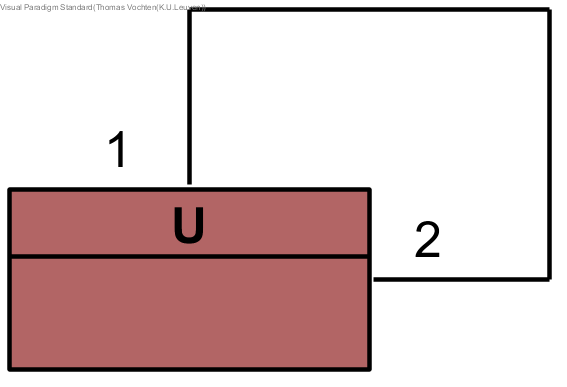
\includegraphics[width=0.6\textwidth]{chap-consistentie/voorbeeld3.png}
		\caption{}
		\label{fig:incon-assoc-simple}
	\end{subfigure}%
	\begin{subfigure}[b]{0.3\textwidth}
		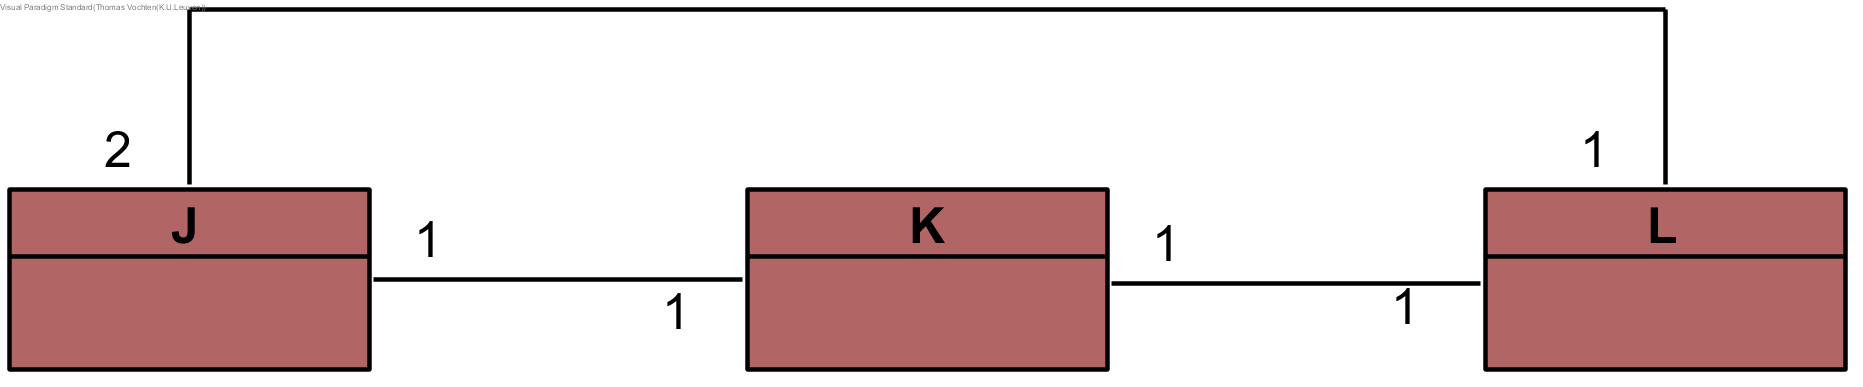
\includegraphics[width=2\textwidth]{chap-consistentie/voorbeeld4.png}
		\caption{}
		\label{fig:incon-assoc-multi}
	\end{subfigure}
	\caption{Voorbeelden van oneindige modellen ten gevolge van associaties}
	\label{fig:incon-assoc}
\end{figure}

\begin{figure}
	\centering
	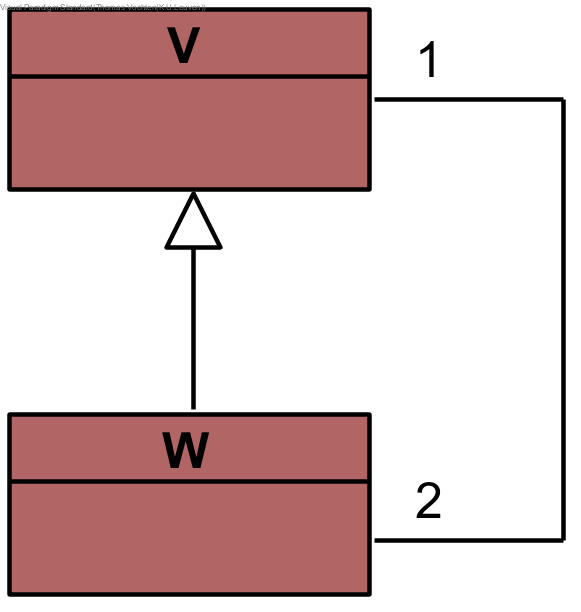
\includegraphics[width=0.175\textwidth]{chap-consistentie/voorbeeld5.png}
	\caption{Voorbeeld van oneindige modellen ten gevolge van een overervingsrelatie en associatie}
	\label{fig:incon-gen-assoc}
\end{figure}

Beschouw het diagram in figuur \ref{fig:incon-assoc-simple}. Stel dat de klasse \textit{U} twee instanties \textit{u1} en \textit{u2} bevat. We proberen de associatie in te vullen als volgt: $\{u1\leftrightarrow{}u1; u1\leftrightarrow{}u2\}$. Om \textit{u2} twee gerelateerde objecten aan de rechterkant te geven, zouden we allereerst $u2\leftrightarrow{}u1$ moeten toevoegen, maar dit zou ingaan tegen de multipliciteit van 1 aan de linkerkant voor \textit{u1}. Voor een gelijkaardige reden kan $u2\leftrightarrow{}u2$ ook niet toegevoegd worden. Zo wordt er afgedwongen dat er twee extra instanties moeten toegevoegd worden: \textit{u3} en \textit{u4}. Zo kunnen we $u2\leftrightarrow{}u3$ en $u2\leftrightarrow{}u4$ toevoegen. Wanneer we \textit{u3} en \textit{u4} allebei twee gerelateerde objecten aan de rechterkant willen geven, doet zich echter een gelijkaardig probleem als voor \textit{u2} voor waardoor de toevoeging van \textit{u3} en \textit{u4} nodig was in de eerste plaats. Dit zorgt ervoor dat een geldig niet-leeg model voor dit diagram oneindig groot zou moeten zijn en dat de klasse \textit{U} inconsistent is.

Beschouw het diagram in figuur \ref{fig:incon-assoc-multi}. De associaties \textit{J}---\textit{K} en \textit{K}---\textit{L} hebben tot gevolg dat \textit{J}, \textit{K} en \textit{L} exact even veel instanties moeten bevatten. De associatie \textit{J}---\textit{L} stelt echter dat alle instanties van klasse \textit{L} in verband moeten staan met twee instanties van klasse \textit{J}. Dit zorgt ook voor oneindig grote niet-lege modellen en dus inconsistentie van het diagram.

Beschouw het diagram in figuur \ref{fig:incon-gen-assoc}. Stel dat klasse \textit{V} als directe instantie \textit{v} heeft en klasse \textit{W} als directe instanties \textit{w1} en \textit{w2}. We stellen $\{v\rightarrow{}w1; v\rightarrow{}w2; w1\rightarrow{}v; w2\rightarrow{}v\}$. \textit{w1} en \textit{w2} zijn echter ook instanties van klasse \textit{V}, waardoor er vier nieuwe objecten nodig zijn om de associatie voor beide objecten te vervullen. Het probleem zet zich voor de vier objecten verder. Dit zorgt weer voor oneindig grote niet-lege modellen en inconsistentie van het diagram.

\section{Voorstellingswijze van klassediagrammen in FO($\cdot$) volgens de voorgestelde semantiek}

Het merendeel van het werk in deze sectie bestaat erin om de methode om klassediagrammen te vertalen naar eerste-orde-predicatenlogica ge\"introduceerd in Daniela Berardi et al.\cite{BerardiDaniela2005RoUc} aan te passen om gebruik te maken van logische types zoals gedefinieerd in FO($\cdot$).

Aan de hand van volgend voorbeeld zullen we illustreren welke regels we gebruiken om een theorie op te bouwen:

\begin{figure}[h]
	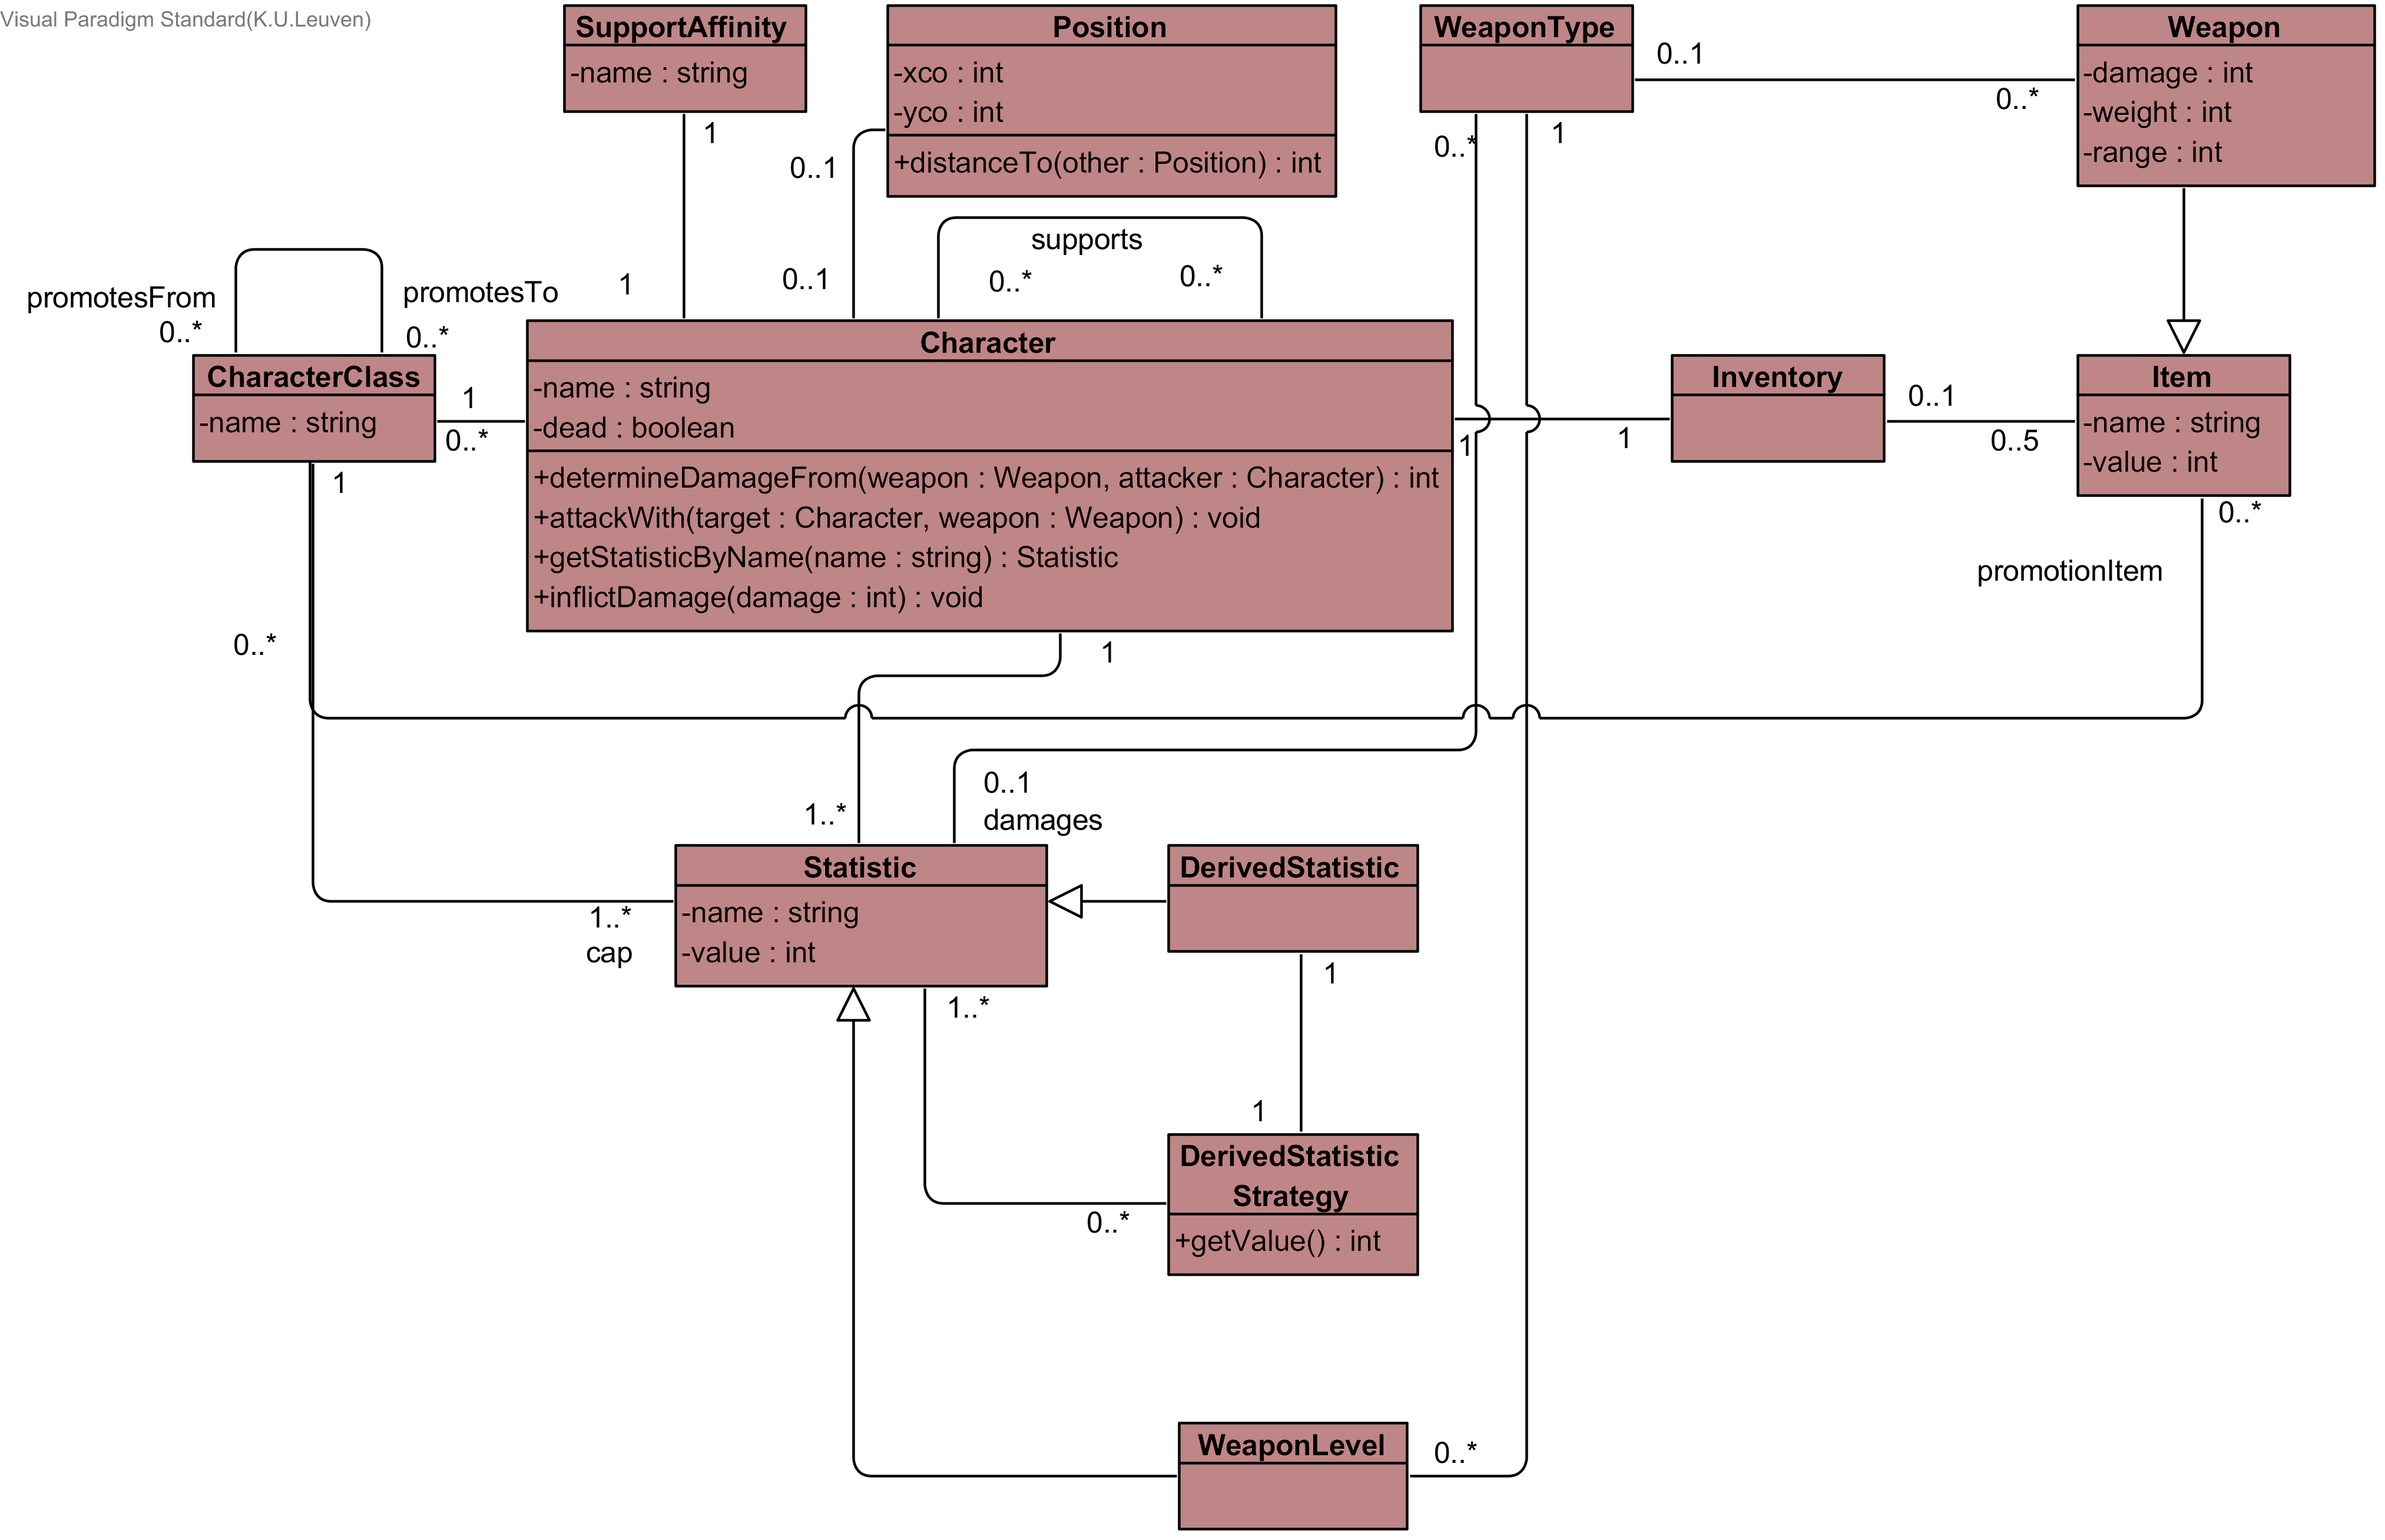
\includegraphics[width=0.95\textwidth]{chap-consistentie/diagram-voorbeeld.png}
	\caption{Leidend voorbeeld van een klassediagram}
	\label{fig:diagram-voorbeeld}
\end{figure}

Meer bepaald willen we uitdrukken welke \textbf{klasses} er bestaan in het diagram waarvan een object een instantie kan zijn, welke \textbf{attributen} en \textbf{operaties} elke klasse bevat, welke \textbf{associaties} er bestaan tussen de verscheidene klasses en welke \textbf{klassehi\"erarchie\"en} er bestaan.

\subsection{Logische types voor objecten}
We moeten een manier hebben om objecten te benoemen in een theorie en te specificeren tot welke klasse die objecten behoren. Voor beide van deze noden zijn logische types geschikt. We voegen voor elke klasse een logisch type toe aan het vocabularium. Er is een logisch type \textit{Character}, een logisch type \textit{Position}, etc.

\subsection{Voorstellen van attributen}
Voor elk attribuut voegen we een binair predicaat toe waarvan de naam beantwoordt aan het patroon: \textit{Klassenaamattribuutnaam}. Voor klasse \textit{Character} en attribuut \textit{name} resulteert dit dus in het predicaat \textit{Charactername/2}. Het eerste argument van dit predicaat is een \textit{Character}. Het type van het tweede argument hangt af van wat er in het diagram staat: Als het een primitief type is zoals \textit{string} of \textit{int}, zal dat ook het type zijn van het tweede predicaat; in het andere geval is het type van het tweede argument het overeenkomstig logisch type voor die klasse. Op deze manier wordt afgedwongen dat elk argument van het predicaat van het juiste type is.
De signatuur van \textit{Charactername/2} is daarom \textit{Charactername(Character, string)}.
Voor elk attribuut wordt ook een regel omtrent multipliciteit afgeleid. Zij \textit{lowerBound} de ondergrens en \textit{upperBound} de bovengrens. Dan is de meest algemene vorm van deze regel als volgt:
	
\begin{align*}
	\forall{o1}[KlasseType](lowerBound \geq \#\{o2 [AttribuutType] : \\ Klassenaamattribuutnaam(o1,o2)\} \geq upperBound).
\end{align*}
	
waarbij \textit{lowerBound} wordt weggelaten als deze $0$ is en \textit{upperBound} wordt weggelaten als deze $*$ is. Indien beide van deze voorwaarden gelden, wordt er geen regel afgeleid betreffende de multipliciteit van het attribuut. Als $lowerBound = upperBound$, wordt deze regel in de plaats:
	
\begin{align*}
	\forall{o1}[KlasseType] \exists_{=upperBound}{o2}[AttribuutType](Klassenaamattribuutnaam(o1,o2)).
\end{align*}
	
Voor \textit{Charactername/2} wordt daarom afgeleid:
	
\begin{align*}
	\forall{o1}[Character]\exists!{x}[string](Charactername(o,x)).
\end{align*}

\subsection{Voorstellen van operaties}
Voor elke operatie voegen we een functie toe dat beantwoordt aan volgend patroon: \sloppy
	 \textit{Klassenaamoperatienaam/(m+1) : ResultaatType}, waarbij $m$ het aantal argumenten dat als invoer wordt meegegeven aan de operatie en \textit{ResultaatType} het type van het resultaat, zij het een primitief type of een klasse. De signatuur ziet eruit als \textit{$Klassenaamoperatienaam(o,p_1,\ldots,p_m)$}, waarbij \textit{o} het object van het logisch type overeenkomstig de klasse waarvan de operatie deel is en \textit{$p_1$} \ldots \textit{$p_m$} de argumenten. Indien er geen argumenten zijn, ziet de signatuur eruit als \textit{Klassenaamoperatienaam(o)}. Voor \textit{determineDamageWeaponFrom(Weapon)} van \textit{Character} wordt dit dus \textit{CharacterdetermineDamageFrom(Character,Weapon) : int}.

Voor elke combinatie van object waarop de operatie wordt opgeroepen en mogelijke invoerparameters moet het het geval zijn dat er \'e\'en enkel resultaat is. Dit is triviaal het geval aangezien een functie elk element uit het domein afbeeldt op exact \'e\'en element uit het codomein.

\subsection{Voorstellen van associaties}
Voor elke associatie voegen we een predicaat toe dat beantwoordt aan volgend patroon: \textit{$ClassOneand\ldots{}andClassM/m$}, waarbij \textit{m} de ariteit van de associatie. Voor de associatie tussen \textit{Inventory} en \textit{Item} wordt dit dus \textit{InventoryandItem(Inventory,Item)}.

De multipliciteit voor elke rol moet worden uitgedrukt. Voor alle $o_l$ waarvoor $1 \leq l \leq m$ wordt een regel toegevoegd van de volgende vorm:\\

Zij $lowerBound_l$ de ondergrens en $upperBound_l$ de bovengrens:
\begin{align*}
	&\forall{c_1}[Klasse_1]\ldots\forall{c_m}[Klasse_m](lowerBound_l \leq
	\\
	&\#\{o_l[Klasse_l] : ClassOneand\ldots{}andClassM(c_1,\ldots,o_l,\ldots,c_m)\} \leq upperBound_l).
\end{align*}
	
waarbij de \textit{c} met index \textit{l} overgeslagen wordt. Indien de ondergrens gelijk is aan $0$ of de bovengrens gelijk is aan $*$ worden deze weggelaten. Als beide voorwaarden gelden, wordt voor deze \textit{l} geen regel afgeleid. Indien $lowerBound_l = upperBound_l$ wordt in de plaats afgeleid:
	
	\begin{align*}
	&\forall{c_1}[Klasse_1]\ldots\forall{c_m}[Klasse_m] \exists_{=upperbound_l}o_l[Klasse_l](ClassOneand\ldots{}andClassM\\&(c_1,\ldots,o_l,\ldots,c_m)).
	\end{align*}
	
	Voor \textit{InventoryandItem/2} worden de volgende regels afgeleid:
	
\begin{align*}
		\forall{o_2}[Item](\#{o_1[Inventory]: InventoryandItem(o_1,o_2)} \leq 1).
\end{align*} 
		
\begin{align*}
		\forall{o_1}[Inventory](\#{o_2[Item]: InventoryandItem(o_1,o_2)} \leq 5).
\end{align*}

\subsection{Voorstellen van klassehi\"erarchi\"een}\label{sec:hierarchies}
Aangezien FO($\cdot$) een getypeerde logica is, is het eenvoudig om klassehi\"erarchie\"een voor te stellen. Als volgens het diagram klasse \textit{X} een subklasse is van klasse \textit{Y}, dan is het voldoende om in het uitvoervocabularium te noteren dat logisch type \textit{Y} een supertype is van logisch type \textit{X}. Het is mogelijk om op die manier een keten van overervingsrelaties te modelleren en zo een hi\"erarchie te verkrijgen. In IDP in het bijzonder is het mogelijk dat een logisch type een subtype is van meer dan \'e\'en type, dus kan men ook meervoudige overerving modelleren.

Dit heeft echter een gevolg voor interpretaties van het logisch type overeenkomstig met een superklasse in een mogelijke structuur volgens het uitvoervocabularium. Indien klasse \textit{Z} een subklasse is van klasse \textit{X} uit de vorige paragraaf, dan moeten alle objecten die behoren tot klasse \textit{Z} ook behoren tot klasse \textit{X}, en zo ook moeten alle objecten die behoren tot klasses \textit{Z} en \textit{X} behoren tot klasse \textit{Y}.

Het is mogelijk om de eindgebruiker dit werk te besparen en automatisch de geschikte interpretaties te laten berekenen door af te stappen van een logisch type voor elke klasse en in de plaats twee nieuwe logische types te introduceren: Een algemeen logisch type voor objecten, \textit{Object}; en een \textit{constructed type}\cite{DeCatBroes2014PLaa} dat voor elke klasse in het diagram een overeenkomstig object heeft, \textit{ClassObject}.

Om lidmaatschap van een klasse uit te drukken, zijn er verder twee nieuwe predicaten nodig: \textit{RuntimeClass(ClassObject, Object)}, wat voor elk object uitdrukt tot welke klasse precies het behoort; en \textit{StaticClass(ClassObject, Object)}, wat uitdrukt tot welke klasses een object behoort als gevolg van de klassehi\"erarchie\"en in het diagram.

Er zijn ook twee predicaten nodig om overervingsrelaties tussen klasses te modelleren: \textit{IsDirectSupertypeOf(ClassObject, ClassObject)} om directe overervingsrelaties voor te stellen; en \textit{IsSupertypeOf(ClassObject, ClassObject)} dat de transitieve sluiting voor \textit{IsDirectSupertypeOf} voorstelt. Aangezien het in predicatenlogica onmogelijk is om een algemene voorstelling voor transitieve sluitingen uit te drukken, maken we gebruik van inductieve definities\cite{DeCatBroes2014PLaa}:

\begin{align}
\{
\nonumber &\forall{x}[ClassObject]\forall{y}[ClassObject](\mathit{IsSupertypeOf}(x,y) \leftarrow \\ &\mathit{IsDirectSupertypeOf}(x,y)).\label{def:tc1} \\
\nonumber &\forall{x}[ClassObject]\forall{y}[ClassObject](\mathit{IsSupertypeOf}(y,x) \leftarrow \\
&\exists{z}(\mathit{IsSupertypeOf(y,z)} \land \mathit{IsSupertypeOf}(z,x))).\label{def:tc2}
\}
\end{align}

\sloppy Zin \ref{def:tc1} maakt gebruik van \textit{IsDirectSupertypeOf/2} om een basisgeval voor \\ \textit{IsSupertypeOf/2} op te stellen. Zin \ref{def:tc2} bouwt dan verder de hi\"erarchie\"en op.

We maken in een tweede definitie gebruik van \textit{IsSupertypeOf/2} om \textit{StaticClass/2} in te vullen:

\begin{align*}
\{
&\forall{x}[ClassObject]\forall{o}[Object](StaticClass(x,o) \leftarrow RuntimeClass(x,o)). \\
&\forall{x}[ClassObject]\forall{y}[ClassObject]\forall{o}[Object](StaticClass(y,o) \leftarrow \\ &RuntimeClass(x,o) \land \mathit{IsSupertypeOf}(y,x)).
\}
\end{align*}

In een aparte definitie lijsten we de invulling voor \textit{IsDirectSupertype/2} gebaseerd op het diagram op. Voor het diagram in figuur \ref{fig:diagram-voorbeeld} wordt dit:

\begin{align*}
\{
&\mathit{IsDirectSupertypeOf}(Statistic,Weaponlevel) \leftarrow .\\
&\mathit{IsDirectSupertypeOf}(Statistic,DerivedStatistic) \leftarrow .\\
&\mathit{IsDirectSupertypeOf}(Item,Weapon) \leftarrow .\\
\}
\end{align*}

We hebben echter niet voor deze aanpak gekozen voor twee redenen.
Attribuutpredicaten, operatiepredicaten en associatiepredicaten zouden logisch type \textit{Object} als argumenten moeten hebben. Dit betekent dat er nieuwe regels nodig zijn die afdwingen dat die objecten van het juiste type zijn. Grotere theorie\"en leiden tot een grotere rekentijd en geheugengebruik bij de uitvoering van redeneertaken.
De multipliciteitsregels zouden ook herschreven moeten worden om gebruik te maken van \textit{StaticClass}. Dit maakt zinnen over de hele lijn langer en zorgt ervoor dat ze moeilijker te begrijpen zijn.

\parbreak

In hoofdstuk \ref{sec:rol-idp} wordt de logische theorie die automatisch gegenereerd werd volgens de regels opgelijst in dit hoofdstuk weergegeven en wordt ook uitgelegd hoe die theorie wordt gebruikt om de consistentie van het diagram te controleren.